
\subsection{XML}
\begin{frame}
 \frametitle{Schemat}
\begin{center}
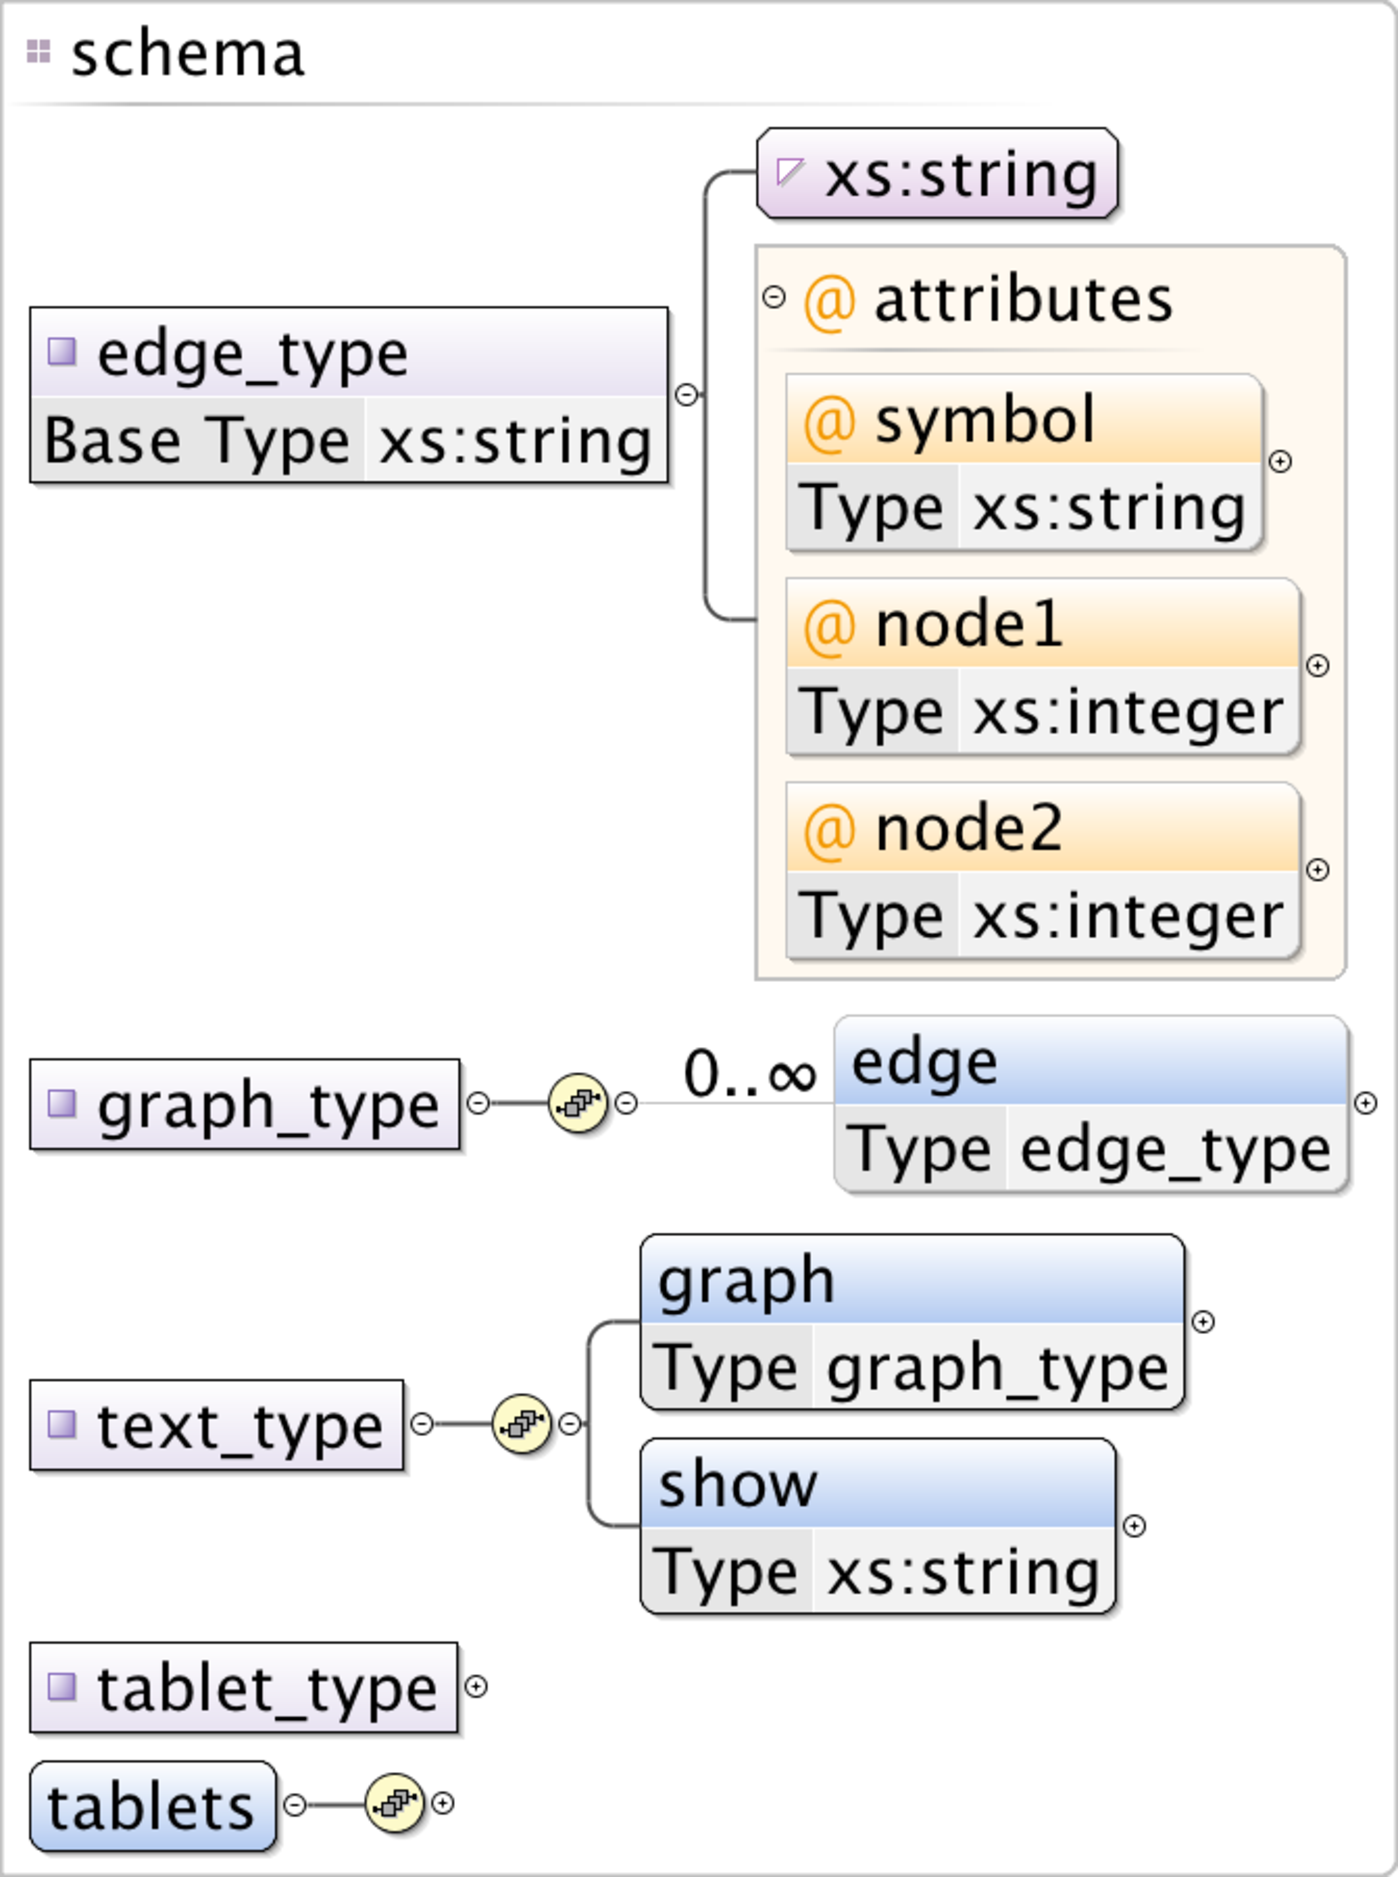
\includegraphics[height=70mm]{../diagramy/schema_text.pdf}
\end{center}

\end{frame}


\begin{frame}
 \frametitle{Schemat}

\begin{columns}[t]
\column{40mm}
\begin{center}
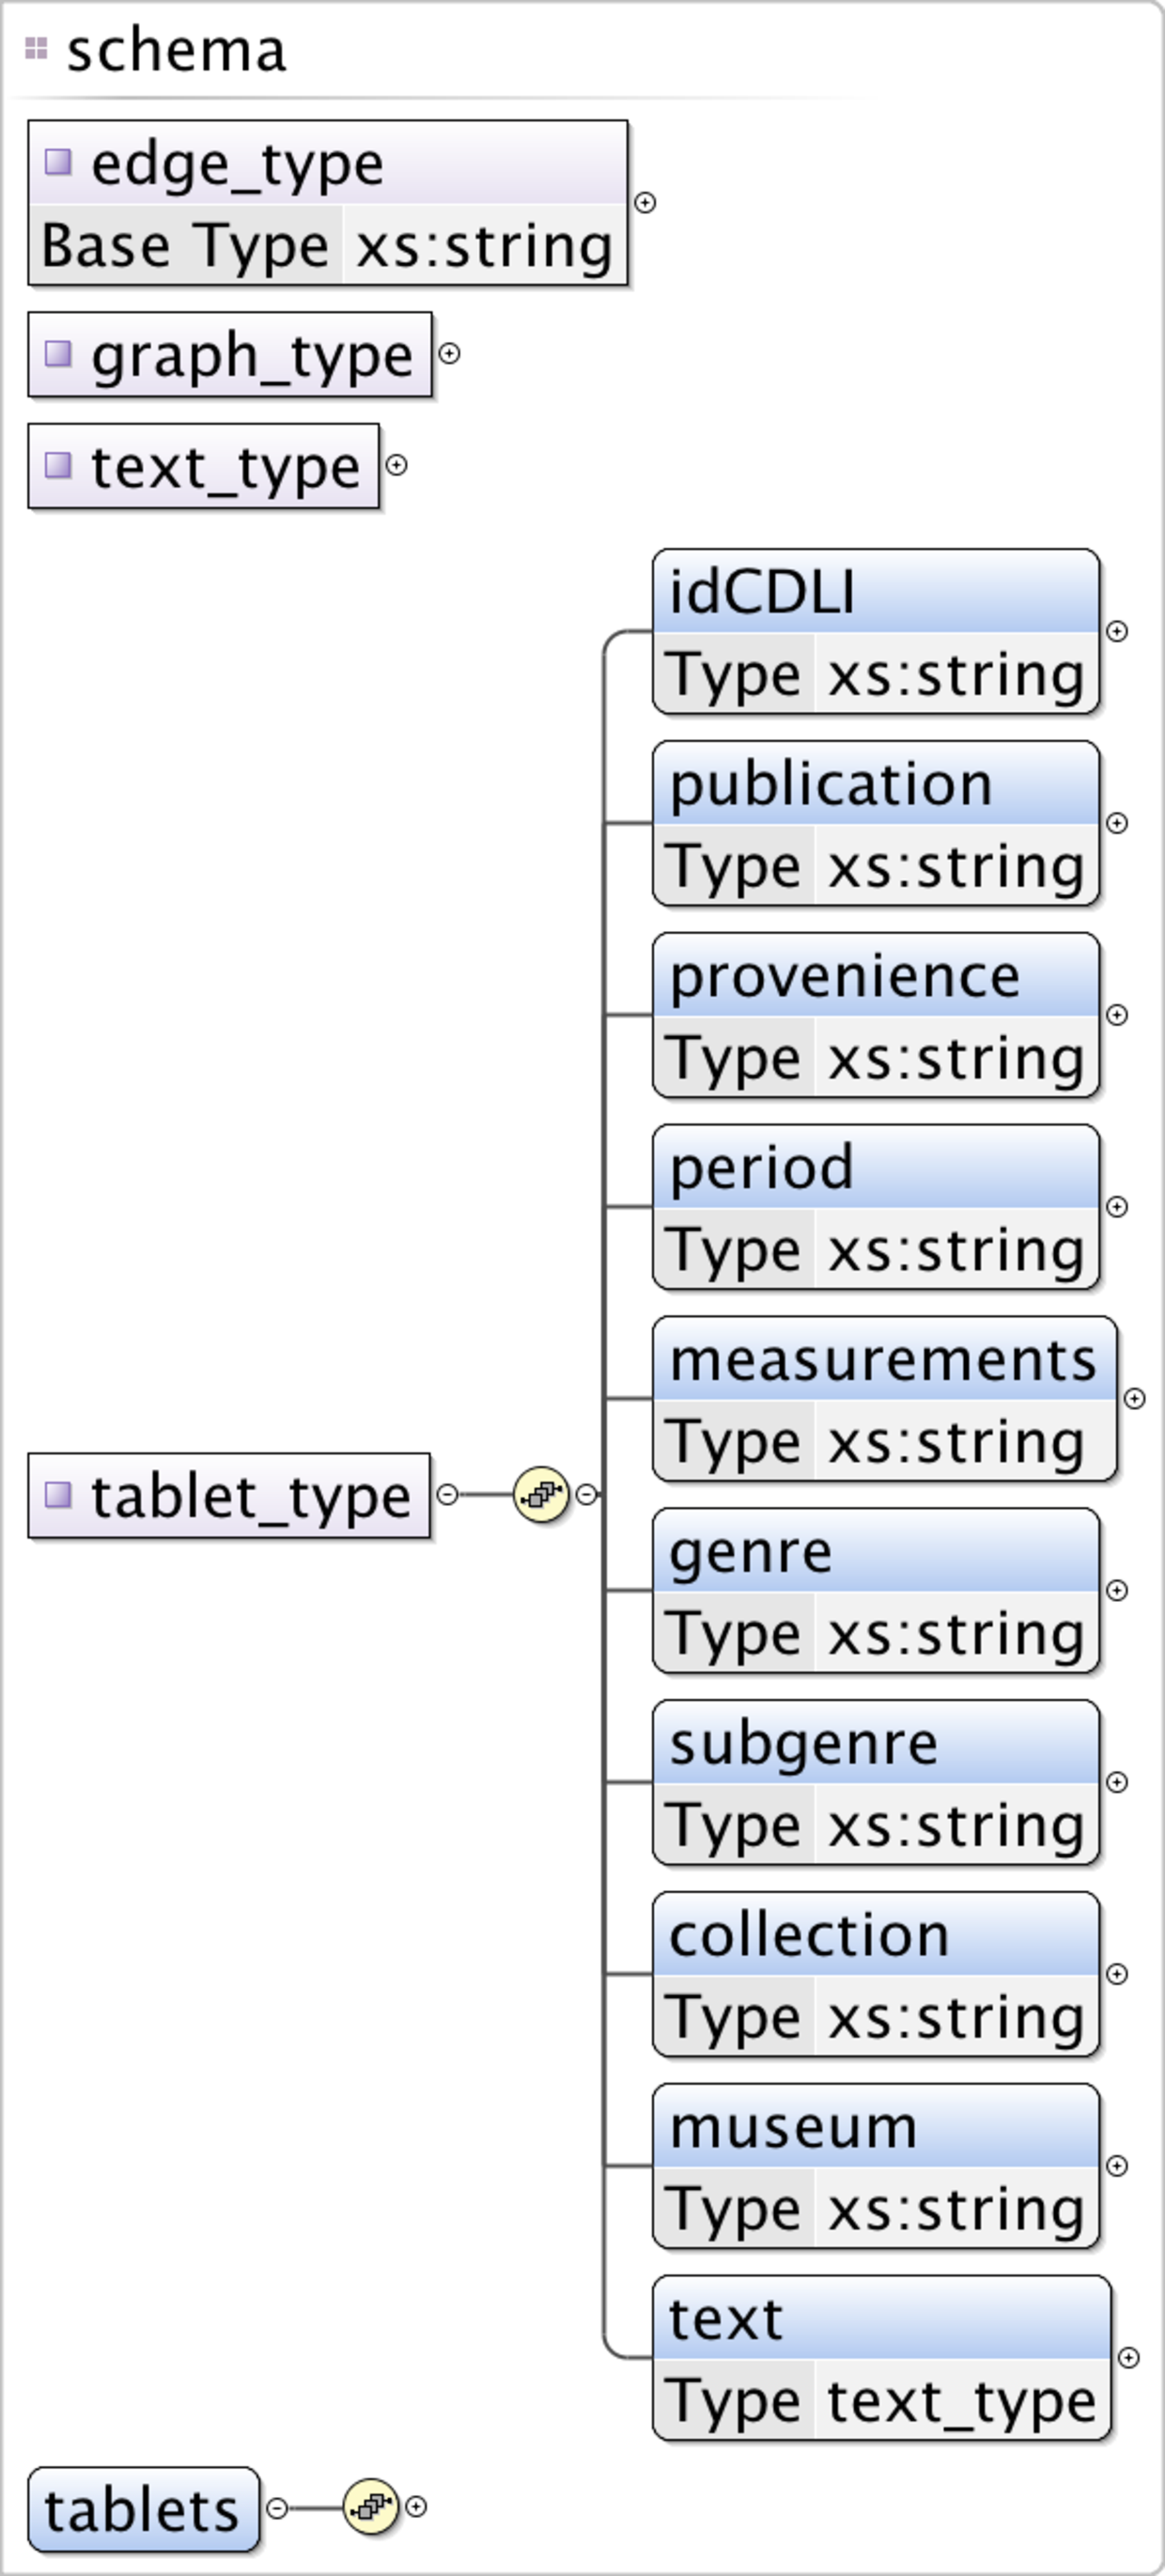
\includegraphics[height=70mm]{../diagramy/schema_tablet.pdf}
\end{center}
\column{40mm}
\begin{center}
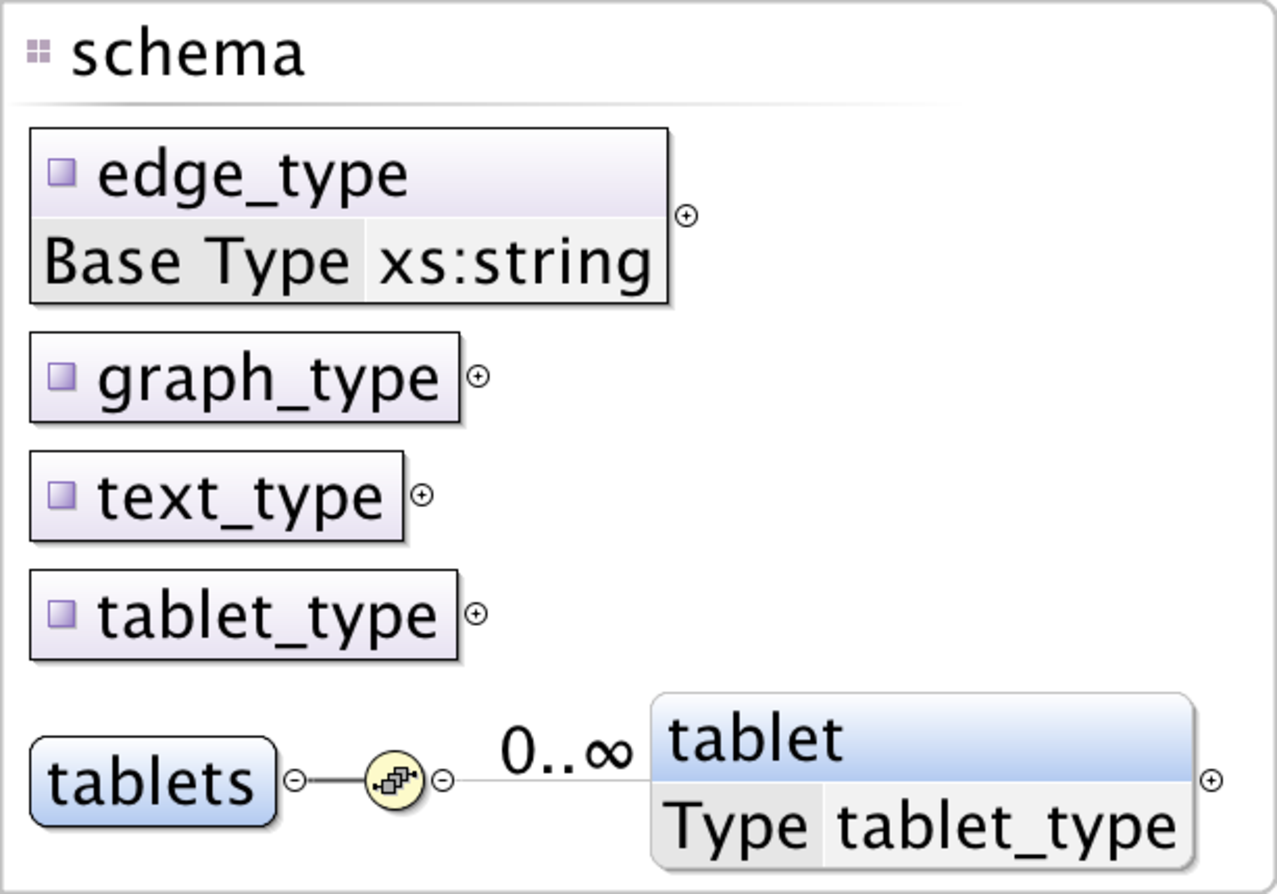
\includegraphics[height=30mm]{../diagramy/schema_tablets.pdf}
\end{center}
\end{columns}

\end{frame}



\begin{frame}
 \frametitle{Tłumaczenie zapytań: stałe fragmenty}
  \begin{block}{For}
	FOR \$tablet IN .//tablet
\end{block}
  \begin{block}{Return}
    RETURN $<$tablet$>$\\
~~{\$tablet/idCDLI}\\
~~{\$tablet/publication}\\
~~{\$tablet/provenience}\\
~~{\$tablet/period}\\
~~{\$tablet/measurements}\\
~~{\$tablet/genre}\\
~~{\$tablet/subgenre}\\
~~{\$tablet/collection}\\
~~{\$tablet/museum}\\
~~{\$tablet/text/show}\\
~~$<$seq$>$...$<$/seq$>$\\
$<$/tablet$>$
\end{block}
\end{frame}

\begin{frame}
	 \frametitle{Tłumaczenie zapytań: zapytania proste}
	\begin{block}{provenience: wartosc}
	fn:matches(\$tablet/provenience,'\textasciicircum wartosc\$')
	\end{block}

	\begin{block}{publication: wartosc}
	fn:matches(\$tablet/publication,'\textasciicircum wartosc\$')
	\end{block}

	\begin{block}{period: wartosc}
	fn:matches(\$tablet/period,'\textasciicircum wartosc\$')
	\end{block}

	\begin{block}{genre: wartosc}
	(fn:matches(\$tablet/genre,'\textasciicircum wartosc\$') or fn:matches(\$tablet/subgenre,'\textasciicircum wartosc\$'))
	\end{block}

	\begin{block}{cdli\_id: wartosc}
	fn:matches(\$tablet/idCDLI,'\textasciicircum wartosc\$')
	\end{block}
\end{frame}

\begin{frame}
 \frametitle{Tłumaczenie zapytań: treść tabliczki}
  \begin{block}{Zapytanie o treść tabliczki}
	let \$seq\textit{$<$id\_sekw$>$} := (\\
  ~~for \$edge\_end in \$tablet//edge\\
  ~~for \$edge\_start in \$tablet//edge\\
~~where (\\
~~~~ fn:matches(\$edge\_start,'\textasciicircum \textit{$<$sekw[0]$>$}\$')\\
~~~~and (\\
~~~~~~some \$edge1 in \$tablet//edge[@node1=\$edge\_start/@node2]\\
~~~~~~~~satisfies (fn:matches(\$edge1,'\textasciicircum \textit{$<$sekw[1]$>$}\$')\\
~~~~~~~~~~and ... \\
~~~~and fn:matches(\$edge\_end,'\textasciicircum \textit{$<$sekw[dl\_sekw-1]$>$}\$')))\\
~~) )\\
return $<$seq\textit{$<$id\_sekw$>$}$>$ {\$edge\_start/@node1} {\$edge\_end/@node2} $<$/seq\textit{$<$id\_sekw$>$}$>$
\end{block}
\begin{block}{where}
	\$seq\textit{$<$id\_sekw$>$}
\end{block}
\end{frame}





\begin{frame}
 \frametitle{Tłumaczenie zapytań: operatory}
\begin{block}{/ -- or}
(\textit{$<$zapytanie1$>$} or \textit{$<$zapytanie2$>$})\\
\end{block}
\begin{block}{+ -- and}
\textit{$<$zapytanie1$>$} and \textit{$<$zapytanie2$>$}\\
\end{block}
\begin{block}{$--$ -- not}
not (\textit{$<$zapytanie\_negowane$>$})\\
\end{block}
\end{frame}

\begin{frame}
 \frametitle{Zorba - procesor XQuery}
\begin{itemize}
\item jest procesorem XQuery, a nie serwerem bazy danych
\item implementuje specyfikacje W3C
\item posiada API do języków: C(?), C++, Ruby, Python, Java, PHP
\end{itemize}
 \end{frame}

